\documentclass{beamer}

% Uncomment for handout
% \documentclass[handout,gray]{beamer}

\usepackage[utf8]{inputenc}
\usepackage{url}
\usepackage{tikz}
\usepackage{pgfplots}
\usetikzlibrary{positioning}
\pgfplotsset{height=5cm,compat=1.9}
\usepackage{graphicx}
\graphicspath{ {images/} }
\usepackage{multicol}
\usetheme{Antibes}

%Information to be included in the title page:
\title[SQAT]{Software Quality Analysis Tools}
\subtitle{SCE15-0367}
\author{Andy Chong Chin Shin\\U1220441H}
\institute[SCSE]{School of Computer Science and Engineering}
\date[FYP, 2016]{Final Year Project Presentation, 2016}
 
\AtBeginSubsection[]
{
  \begin{frame}<beamer>
  \frametitle{Table of Contents}
  \begin{multicols}{2}
  \tableofcontents[currentsubsection]
  \end{multicols}
  \end{frame}
}

\AtBeginSection[]
{
  \begin{frame}<beamer>
  \frametitle{Table of Contents}
  \begin{multicols}{2}
  \tableofcontents[currentsection]
  \end{multicols}
  \end{frame}
}

\begin{document}

\frame{\titlepage}

\begin{frame}
\frametitle{Table of Contents}
\begin{multicols}{2}
\tableofcontents
\end{multicols}
\end{frame}
 
\section{Introduction}
\begin{frame}
\frametitle{Introduction}

Students submit codes to complete exercises, assignments and projects in NTU. Most of the time:

\begin{itemize}
  \item Assignments are assessed based on reports only
  \item Codes are not assessed
\end{itemize} \pause

Infeasible to assess codes because we lack of:

\begin{itemize}
  \item Objectives
  \item Human resources
\end{itemize}
\end{frame}

% ==============================
\subsection{Objective}
\begin{frame}
\frametitle{Objective}

\begin{block}{Long-term Goal}
To develop Software Quality Analysis Tools (SQAT), a tool that is able to assess the quality of the source codes automatically.
\end{block} \pause

SQAT will asses the quality of source codes by considering the structural metrics:

\begin{itemize}
  \item Object-oriented metrics
  \item Coding standards
\end{itemize}
\end{frame}

% ==============================
\subsection{Scope}
\begin{frame}
\frametitle{Scope}

Since this project was started from scratch, in this project, we:

\begin{itemize}
  \item determine a scalable architecture
  \item built software quality measurement tool
  \item built a front-end web application
\end{itemize}

\end{frame}
\section{Literature Review}

\subsection{Software Quality}
\begin{frame}
\frametitle{Software Quality}

\begin{definition}
Software quality is the degree to which software possesses a desired combination of attributes (IEEE, 1998). The desired attributes are called \emph{software quality attributes}.
\end{definition} \pause

\begin{example}
\begin{itemize}
  \item Maintainability
  \item Efficiency
  \item Reliability
\end{itemize}
\end{example}

\end{frame}

\subsection{Software Quality Metric}
\begin{frame}
\frametitle{Software Quality Metric}

We have many software quality metrics.

\begin{example}
\begin{itemize}
  \item Weighted methods per class
  \item Depth of inheritance tree
  \item Coupling factor
\end{itemize}
\end{example}

\end{frame}

\subsection{Goal Question Metric}
\begin{frame}
\frametitle{Goal Question Metric}

We use Goal Question Metric (GQM) to relate software quality metrics (quanlitative) to software quality attributes (quantitative).

\begin{definition}
Goal Question Metrics is a goal oriented data collection for collecting valid software engineering data. (Basili and Weiss, 1984)
\end{definition} \pause

\begin{example}
\begin{tabular}{ l l }
Goal &: Analysability \\
Question &: Are the conditional statements not deep? \\
Metrics &: Depth of conditional nesting\\
Score &: 90\%\\
\end{tabular}
\end{example}

\end{frame}

\subsection{Existing Tool: SonarQube}
\begin{frame}[allowframebreaks]
\frametitle{Existing Tool: SonarQube}

\begin{columns}
\column{0.5\textwidth}
SonarQube is a continuous code inspection tool. Features:
\begin{itemize}
  \item Object-oriented metrics
  \item Code style checking
  \item Code duplication detection
  \item Custom configurations for different projects
  \item Support 20 programming languages
\end{itemize}
\column{0.5\textwidth}
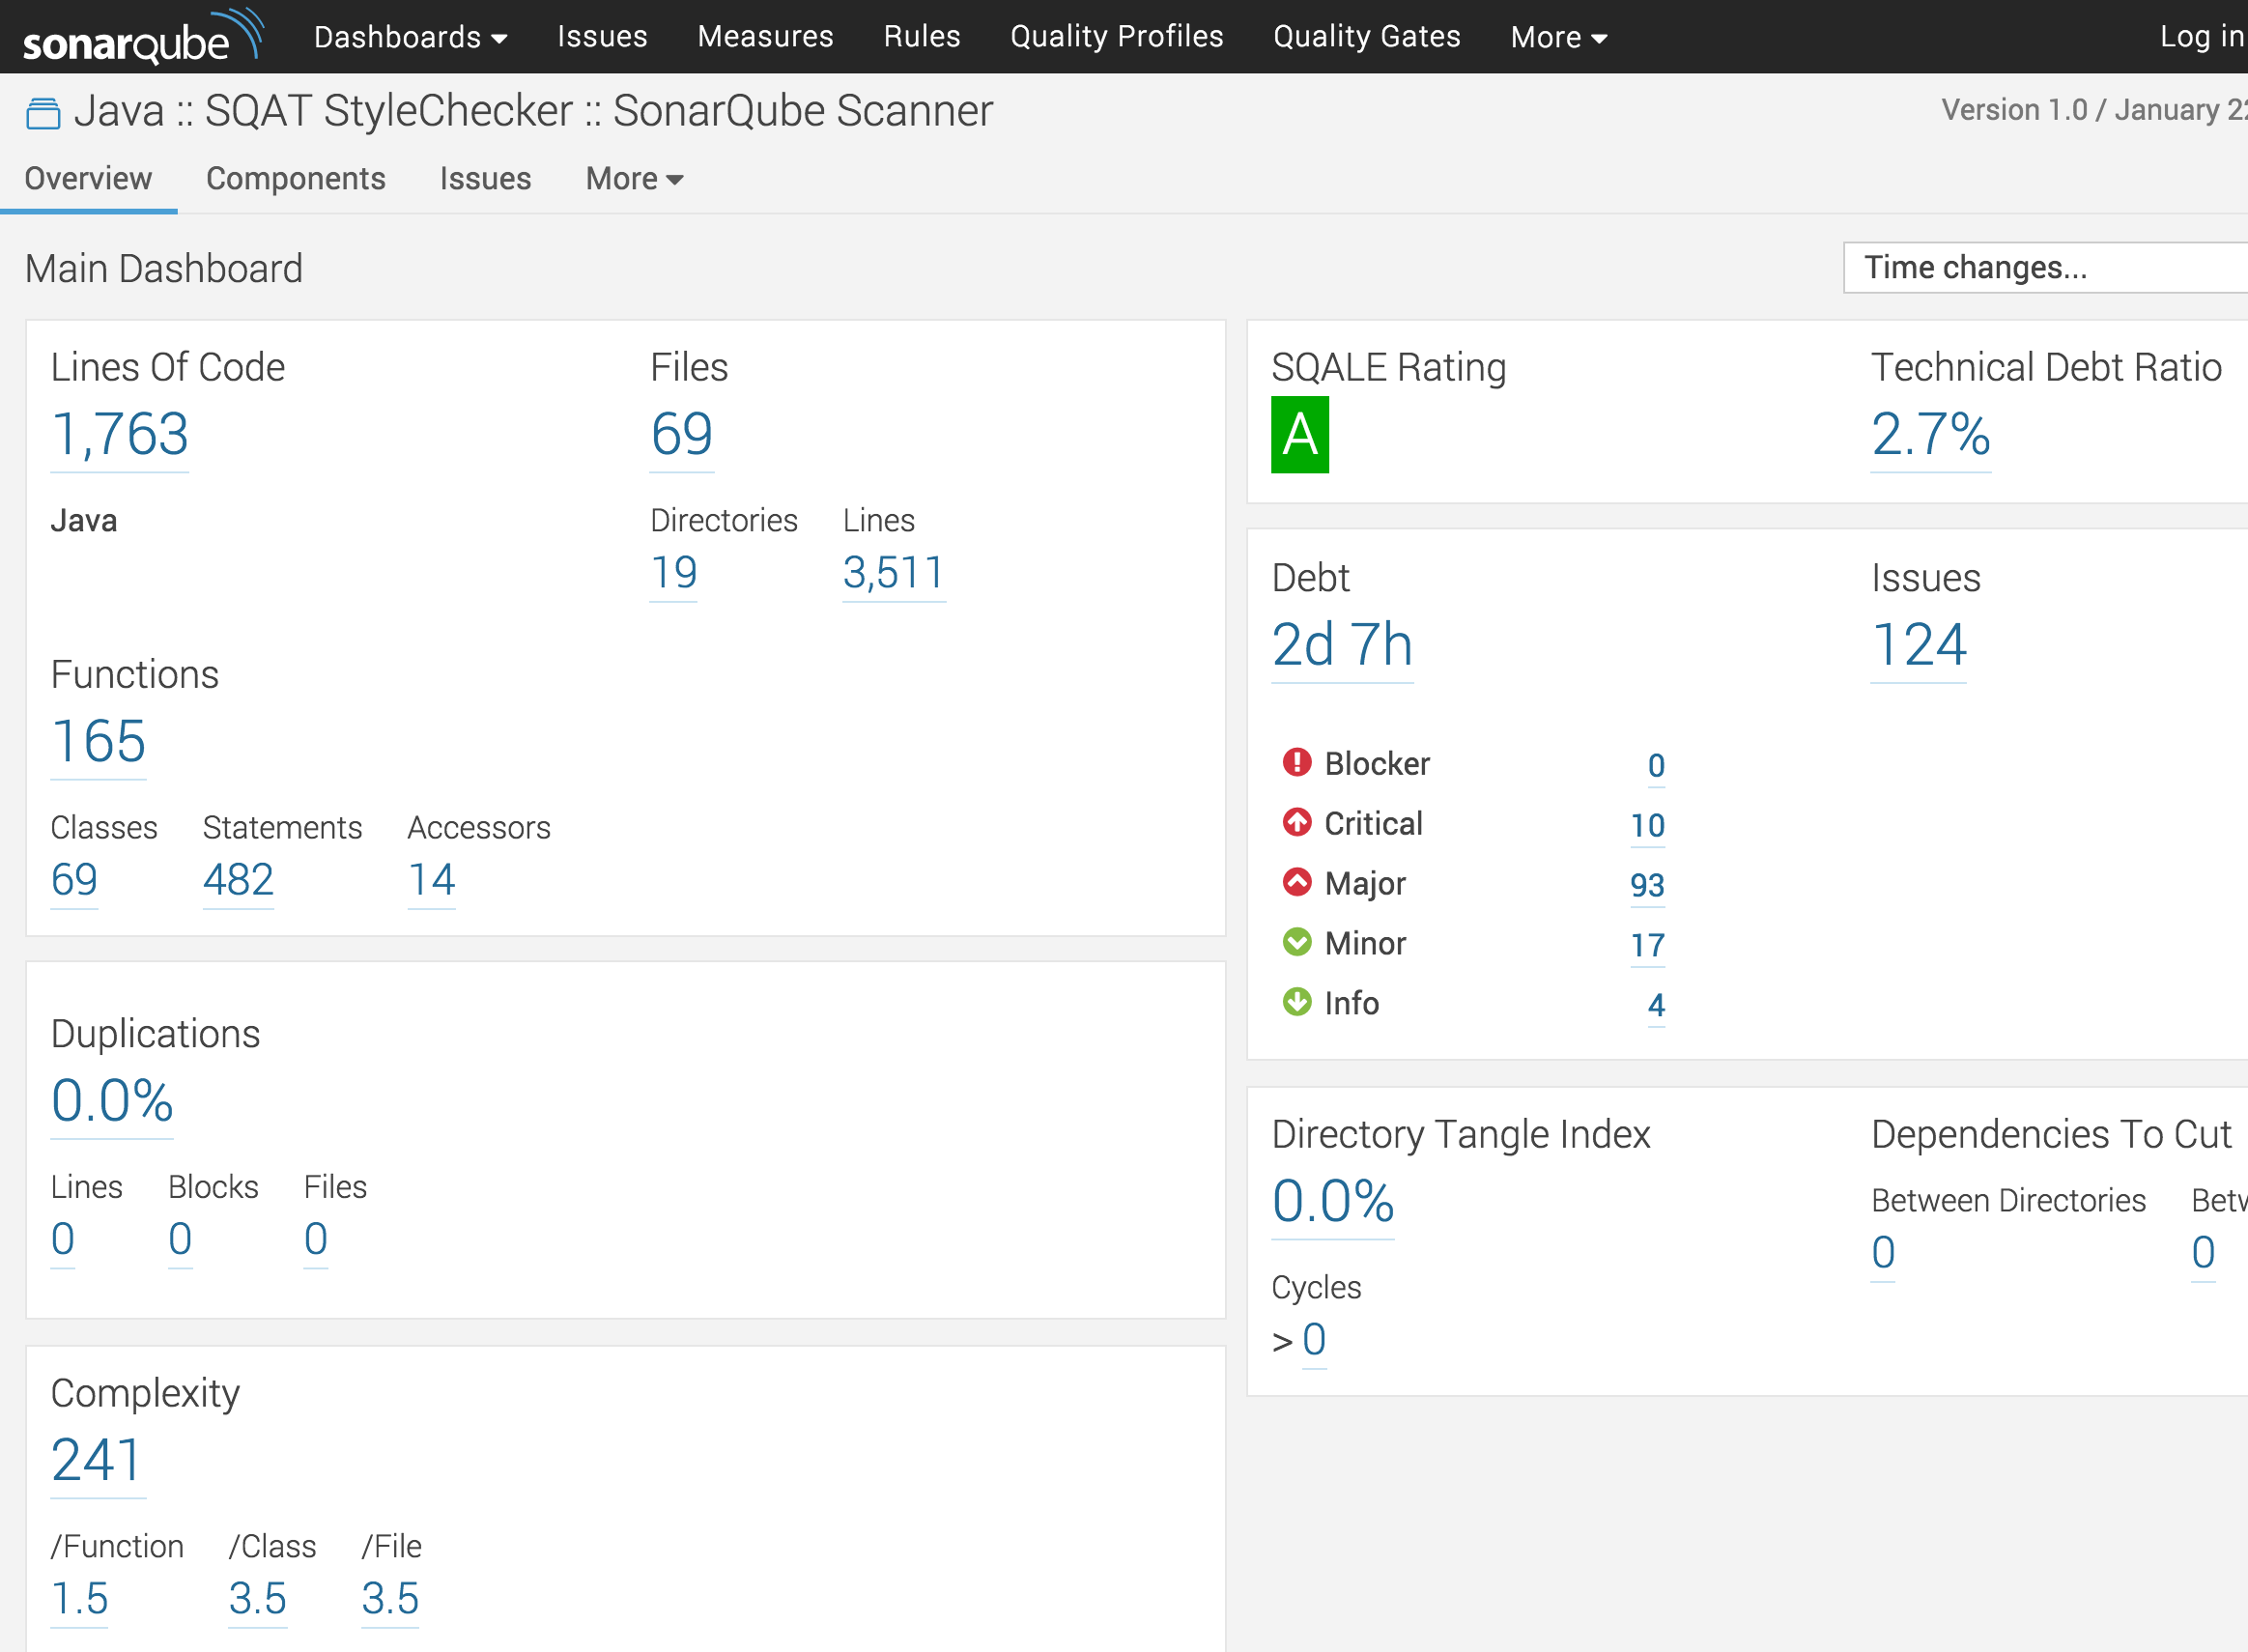
\includegraphics[scale=0.1]{sonar_project_dashboard}
\end{columns}

\framebreak

We do not use SonarQube because:
\begin{itemize}
  \item Need to develop SonarQube plug-in
  \item Do not provide complete API to work with plug-in
    \item Two projects with different goals
  \begin{itemize}
    \item Has user interface for monitoring
    \item Do not have automation tools
  \end{itemize}
\end{itemize}

We decided to develop SQAT from scratch.

\end{frame}
\section{Use Cases}
\begin{frame}
\frametitle{Use Cases}

Students:
\begin{itemize}
  \item Submit source code for quality report
  \item Submit source code for assignment
  \item Check assignment results
  \item Setup SQAT continuous integration
  \item Perform quality assessment request from GitHub Webhook
\end{itemize}

Professors:
\begin{itemize}
  \item Create new assignment for submission
  \item Check student results
\end{itemize}
\end{frame}

\section{Design}

\subsection{ANTLR}
\begin{frame}
\frametitle{ANTLR}

We use ANTLR to generate a parse tree and walk the parse tree to \emph{collect software quality metrics}.

\begin{definition}
ANTLR (ANother Tool for Language Recognition) is a powerful parser generator for reading, processing, executing, or translating structured text or binary files. (Parr, 2013)
\end{definition}

It can \emph{support multiple programming languages}, as long as you define the language structure using a grammar file\footnote{Open source grammar files: https://github.com/antlr/grammars-v4}.

\end{frame}

\subsection{Architecture for Measurement Component}
\begin{frame}
\frametitle{Architecture for Measurement Component}

\only<1>{

Washizaki et al. (2007) proposed a framework that achieves effective measurement and evaluation of source code quality.

\begin{center}
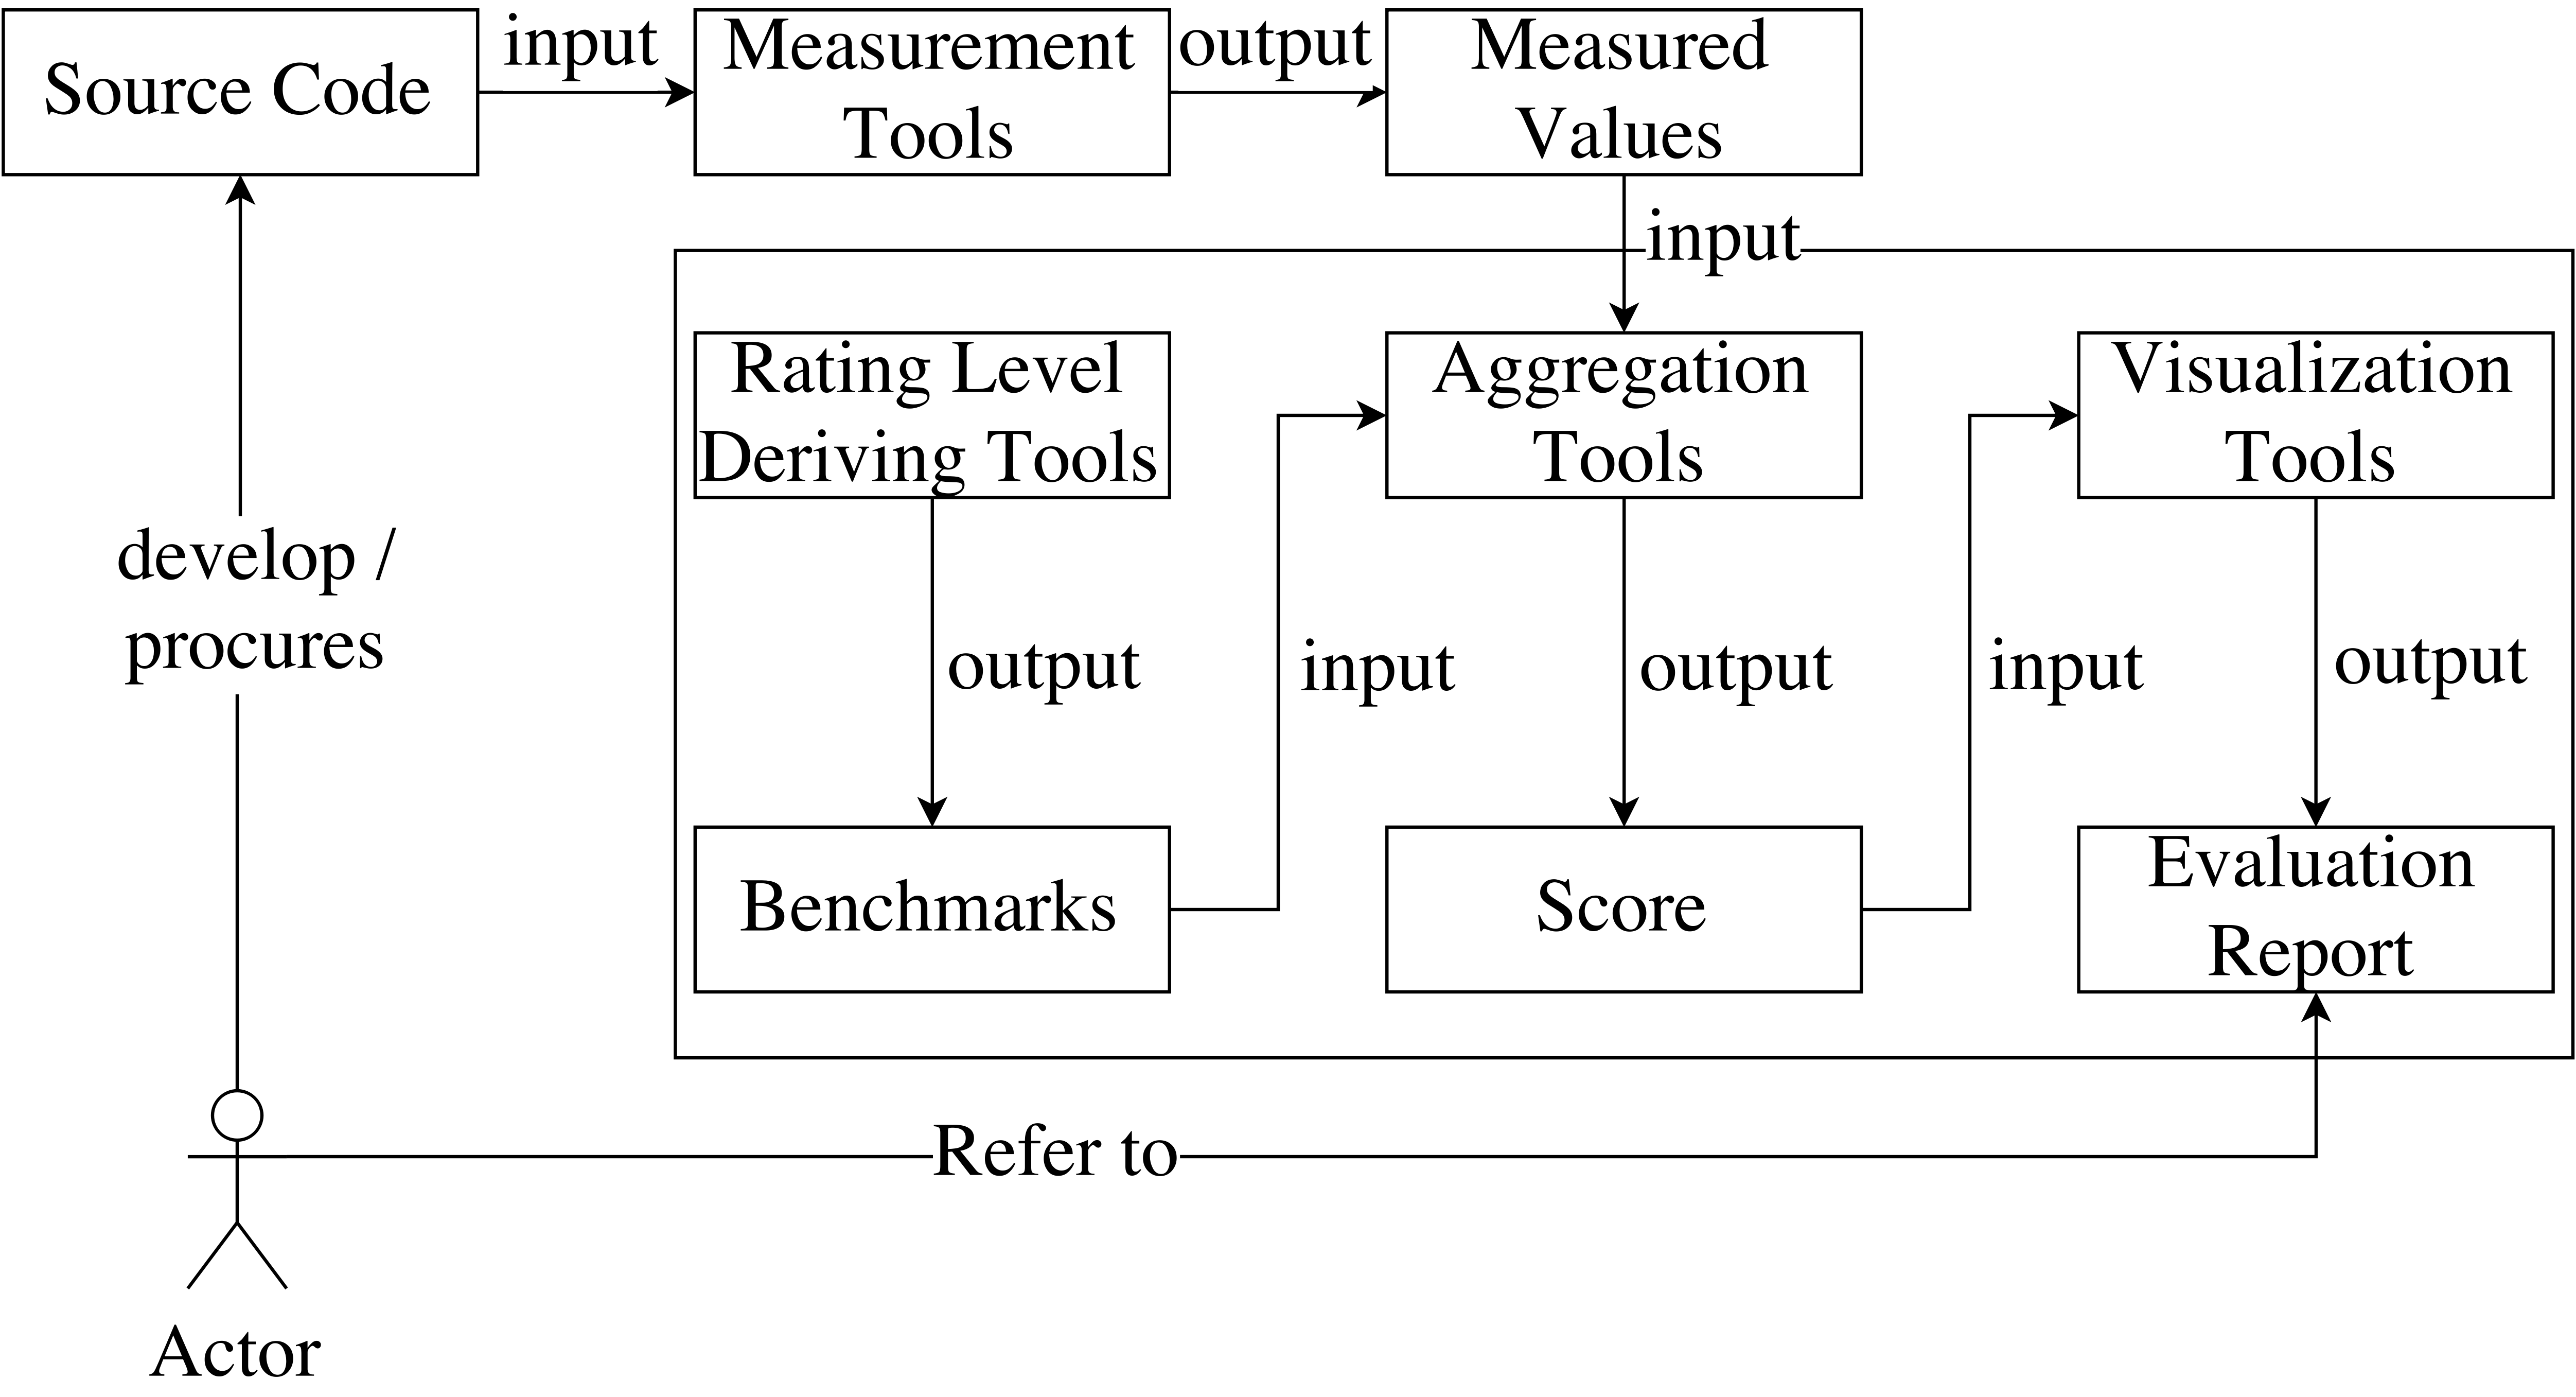
\includegraphics[scale=0.06]{washizaki_framework}
\end{center}
}

\only<2>{

We use the proposed framework to build the measurement component of SQAT.

\begin{center}
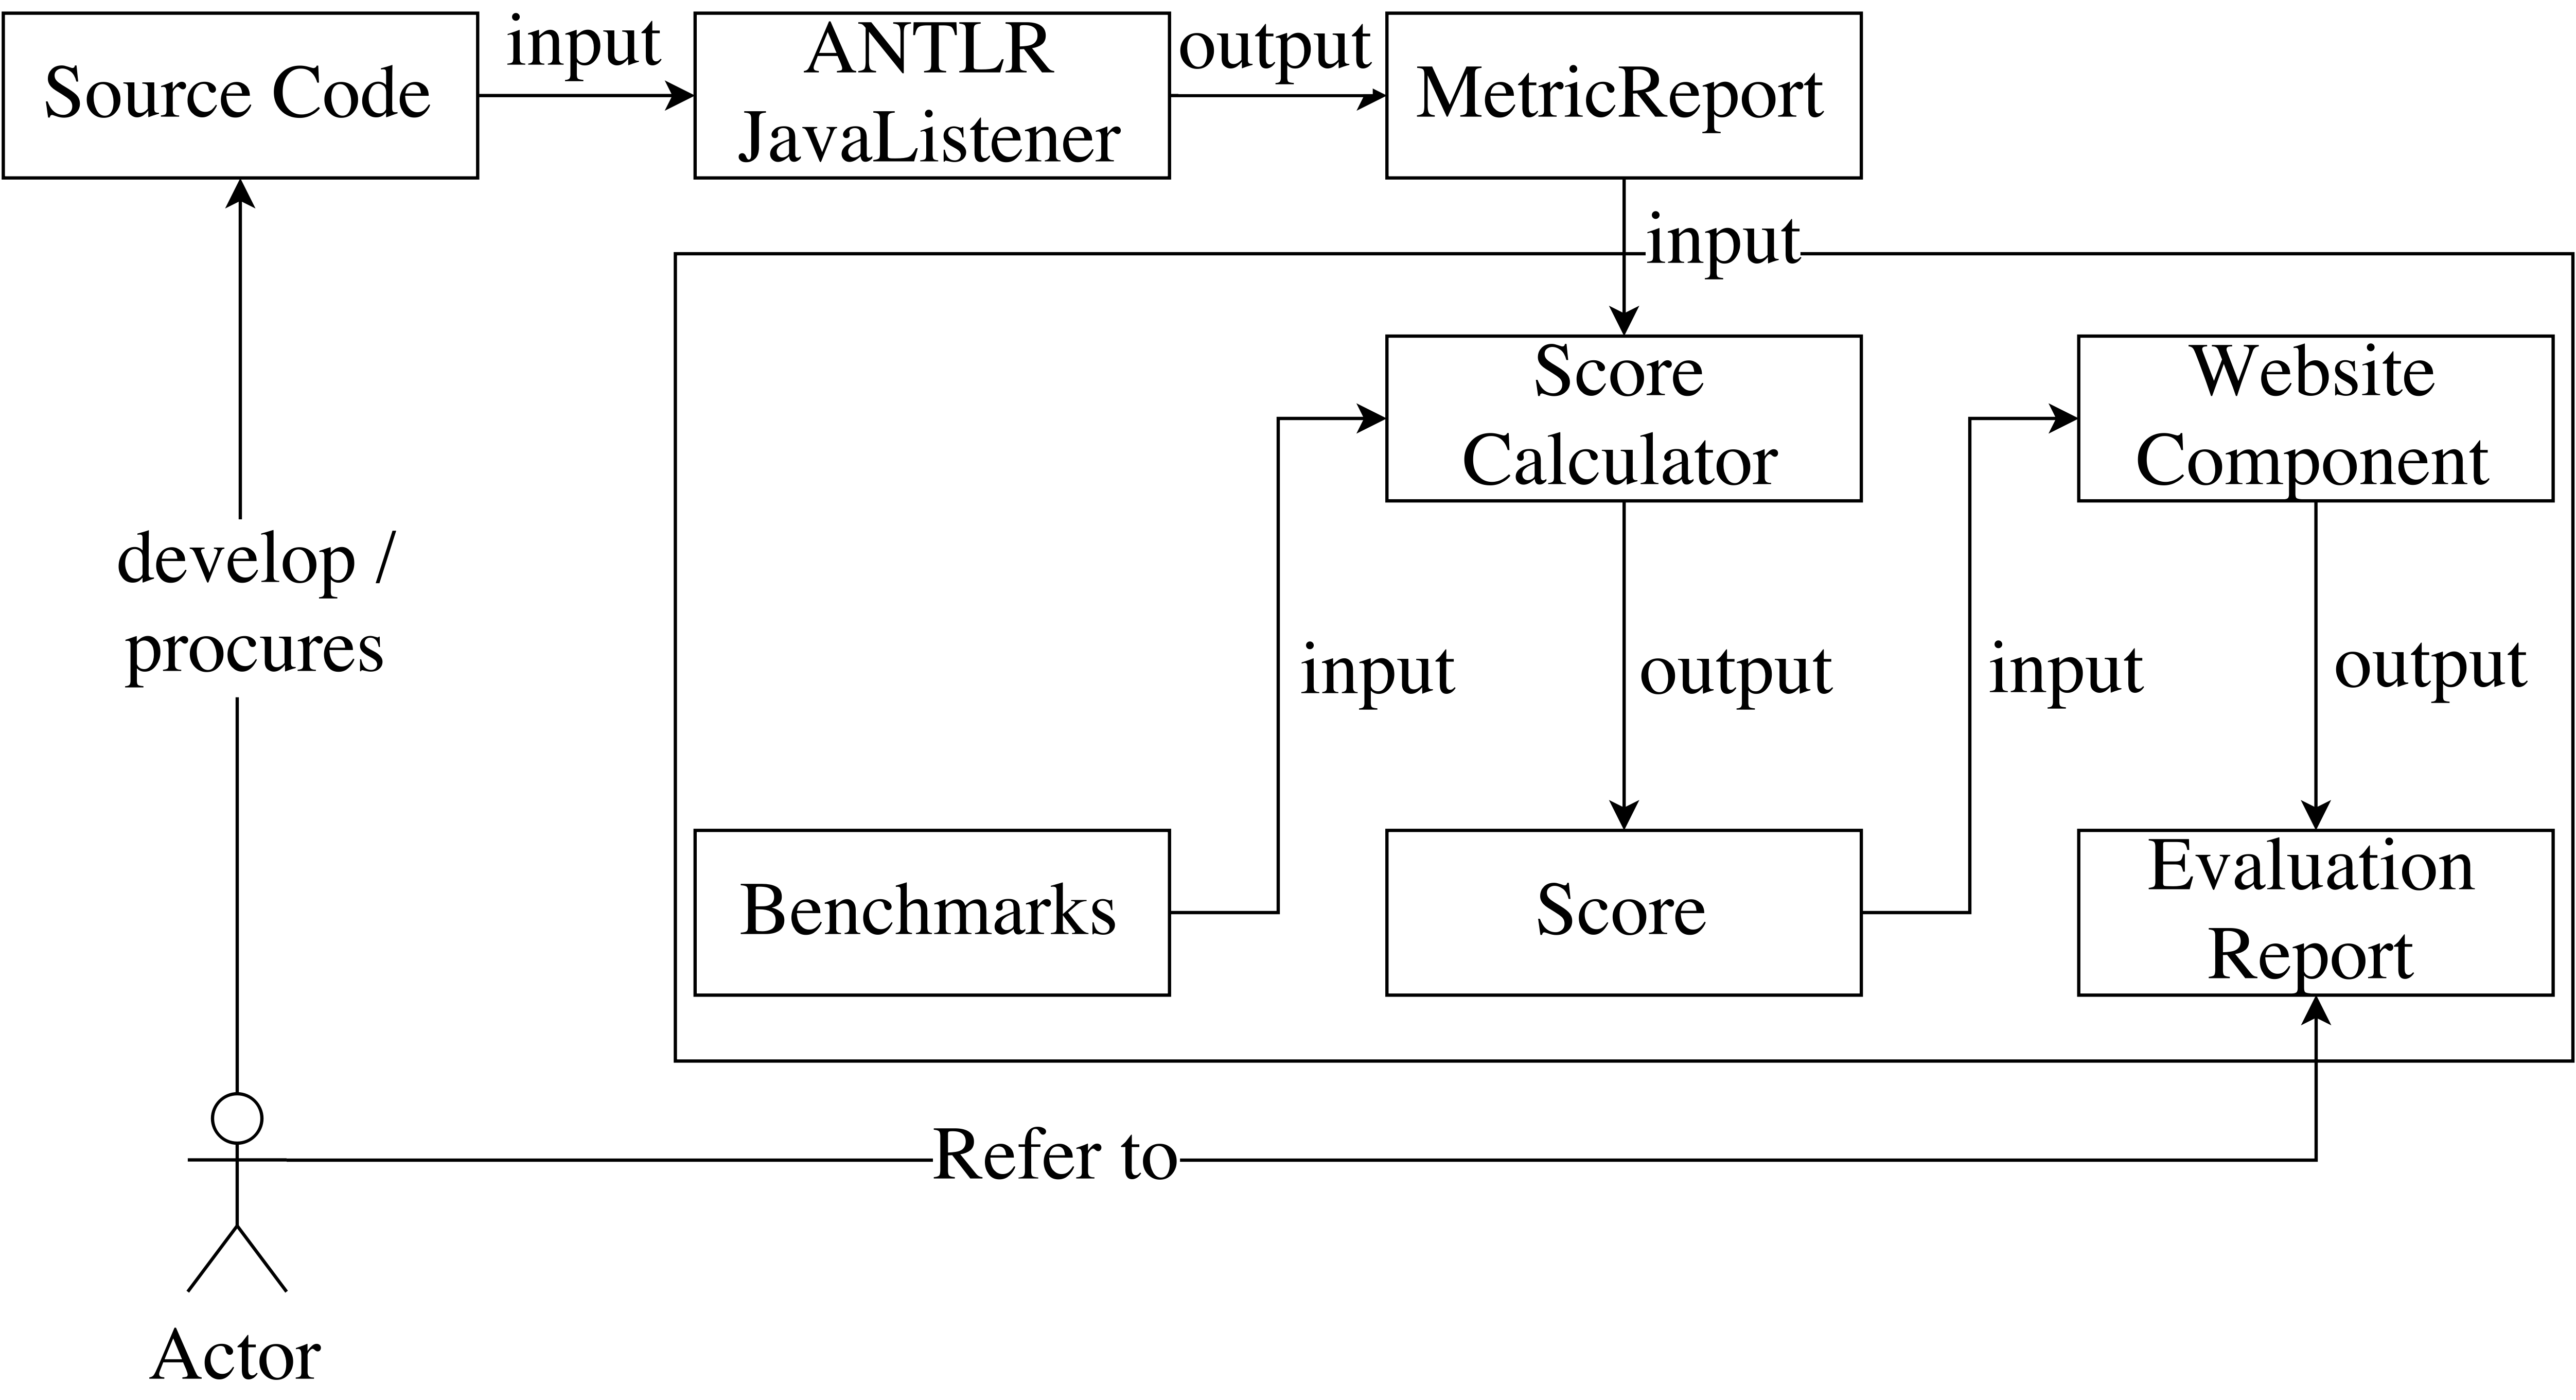
\includegraphics[scale=0.06]{software_quality_measurement_framework}
\end{center}
}
\end{frame}

\section{Implementation}

\subsection{Code Style Configuration}
\begin{frame}[allowframebreaks]
\frametitle{Code Style Configuration}

The measurement component enforces some code styles:

\begin{itemize}
  \item Indentation levels
  \item Import statement styles
  \item Method name format
\end{itemize}

The code style is configurable using a JSON file:

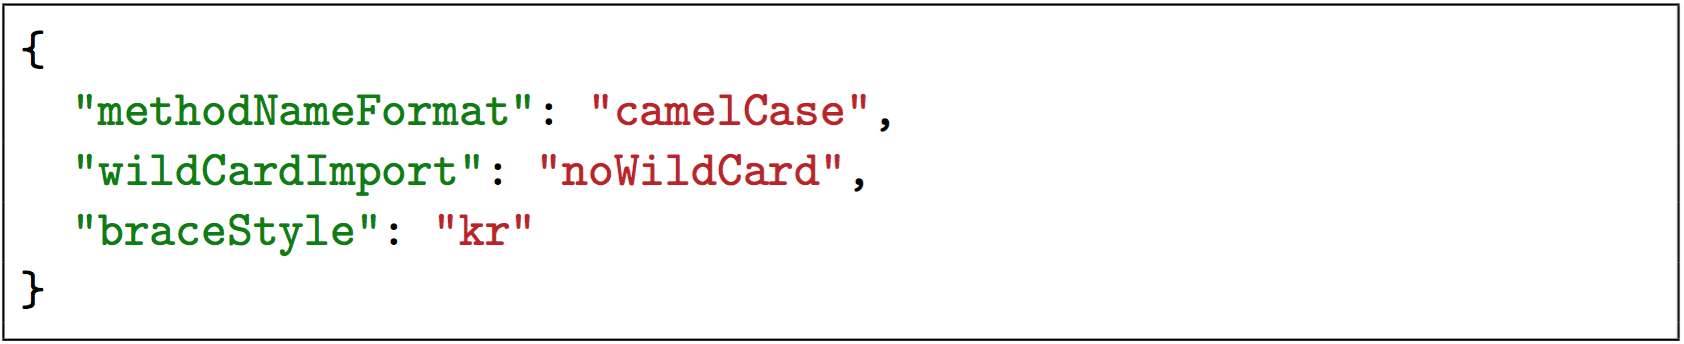
\includegraphics[scale=0.37]{json_config}

\framebreak

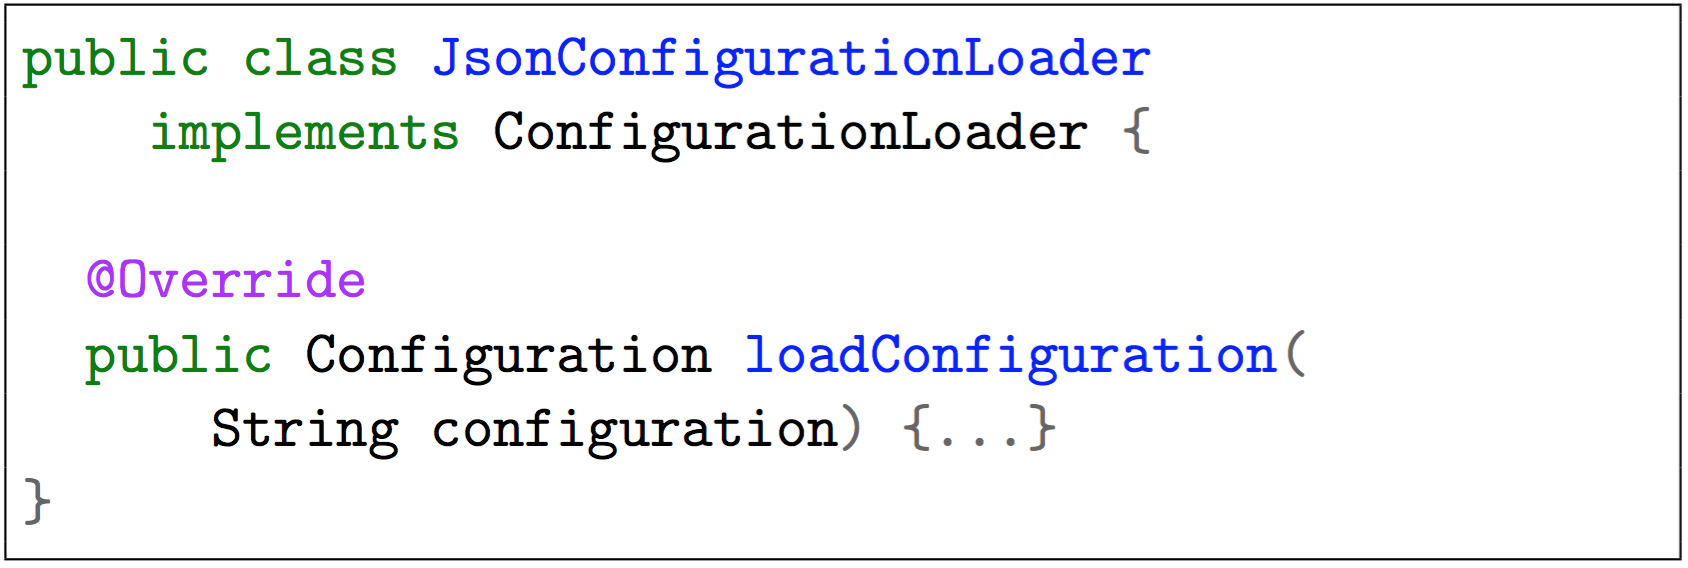
\includegraphics[scale=0.37]{json_configuration_loader}

Measurement component uses \textit{JsonConfigurationLoader} to convert the configuration in \textit{String} to \textit{Configuration} object.

We can implement the \textit{ConfigurationLoader} to support configuration XML and CSV formats.
\end{frame}

\subsection{Score Calculator}
\begin{frame}
\frametitle{Score Calculator}
\setbeamercovered{transparent}

\begin{columns}
\column{0.5\textwidth}
Washizaki et al. (2007) calculate scores based on \emph{benchmark} values and \emph{collected} values by using a linear piecewise function:
\begin{itemize}
  \item<1,4> If the collected value is less than benchmark value, the score is 100\%
  \item<2,4> If the collected value is more than benchmark value and less than 3 times of benchmark, the score is: $$score=\bigg(-\frac{1}{3 \times benchmark} \times value + \frac{4}{3}\bigg) \times 100\%$$
  \item<3,4> Else, the score is zero
\end{itemize}

\column{0.5\textwidth}
\begin{tikzpicture}
\begin{axis}[
    axis lines = left,
    xlabel = value,
    ylabel = score,
]
\addplot [
    domain=1:4, 
    samples=2,
    color=red,
]
{- x/3 + 4/3 };
\addplot [
    domain=0:1, 
    samples=2,
    color=red,
]
{1};
\addplot [
    domain=4:5, 
    samples=2,
    color=red,
]
{0};
\addplot [
    domain=0:1, 
    samples=2, 
    color=white,
]
{1.1};
\end{axis}
\end{tikzpicture}

\end{columns}

\end{frame}

\subsection{Front-end Development}
\begin{frame}
\frametitle{Front-end Development}
To enhance user experience, we built a single page application for front-end of SQAT:
\begin{itemize}
  \item Contents are loaded dynamically using Javascript
  \item URL is changed to emulate traditional navigation
\end{itemize}

We uses Flux Architecture for front-end application:

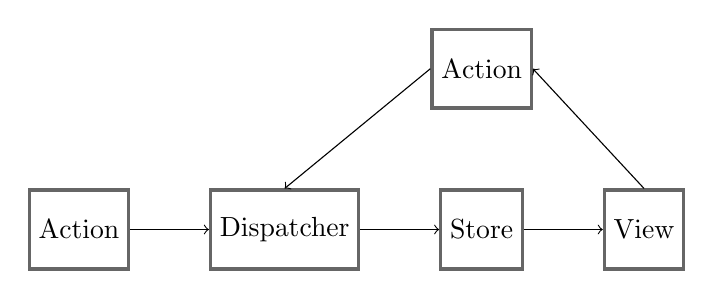
\begin{tikzpicture}[
squarednode/.style={rectangle, draw=black!60, very thick, minimum size=1cm},
]
%Nodes
\node[squarednode](action){Action};
\node[squarednode](dispatcher)[right=of action]{Dispatcher};
\node[squarednode](store)[right=of dispatcher]{Store};
\node[squarednode](view)[right=of store]{View};

\node[squarednode](action2)[above=of store]{Action};

%Lines
\draw[->] (action.east) -- (dispatcher.west);
\draw[->] (dispatcher.east) -- (store.west);
\draw[->] (store.east) -- (view.west);

\draw[->] (view.north) -- (action2.east);
\draw[->] (action2.west) -- (dispatcher.north);
\end{tikzpicture}

\end{frame}
\section{Testing}

\subsection{Continous Testing}
\begin{frame}
\frametitle{Continuous Testing}

\begin{definition}
Continuous testing uses excess cycles on a developer’s workstation to continuously run regression tests in the background, providing rapid feedback about test failures as code is edited (Saff and Ernst, 2005).
\end{definition}

We use continuous testing and Test-driven Development approach to develop SQAT.

\end{frame}

\subsection{Travis CI and Coverall}
\begin{frame}
\frametitle{Travis CI and Coverall}

\only<1>{
  \begin{center}
  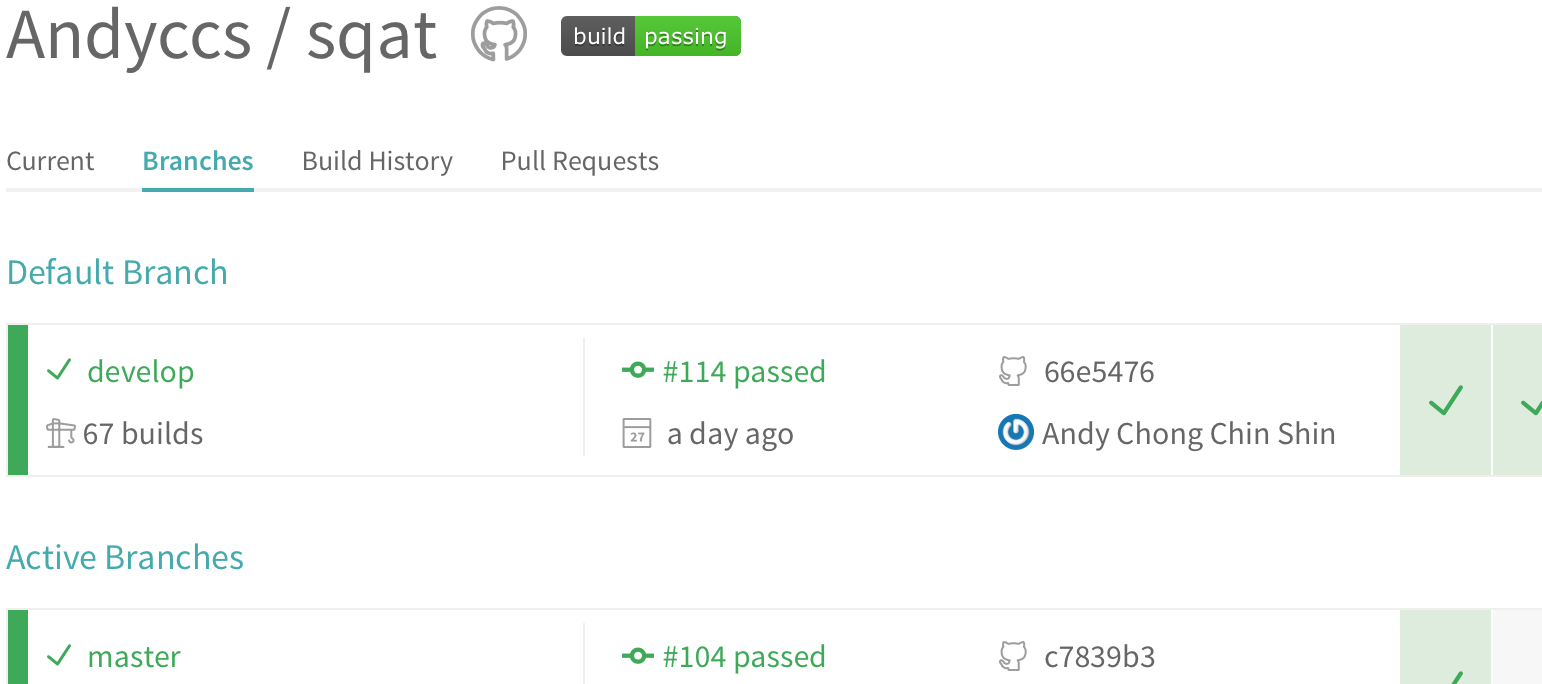
\includegraphics[scale=0.36]{travis_ci}
  \end{center}

  When we check in codes to SQAT code repository, Travis CI will build and test the codes immediately.

  \tiny{\url{Source: https://travis-ci.org/Andyccs/sqat}}
}
\only<2>{
  \begin{center}
  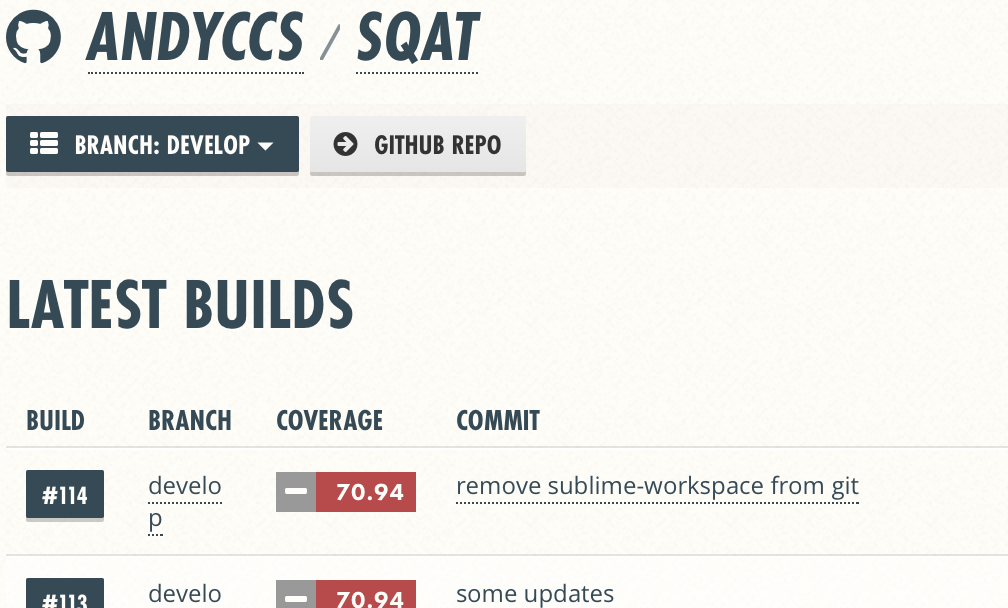
\includegraphics[scale=0.36]{coverall}
  \end{center}

  Similary, Coverall will run all test cases in the repository an generate a code coverage report. 

  \tiny{\url{Source: https://coveralls.io/github/Andyccs/sqat}}
}
\end{frame}
\section{Conclusion}

\begin{frame}
\frametitle{Conclusion}
We have developed the foundation of SQAT:
\begin{itemize}
  \item Identify the main goal is to build an automatic code assessment tool
  \item Use Goal Question Metric approach to quantify software quality attributes
  \item Use ANTLR as the main tool to collect software metrics
  \item Use microservices architecture to develop SQAT
  \item Implement the framework proposed by Washizaki et al. (2007) for measurement component
\end{itemize}

\end{frame}

\subsection{Future Recommendation}
\begin{frame}
\frametitle{Future Recommendation}

SQAT can be further improved in five ways:
\begin{itemize}
  \item Conducting acceptance testing
  \item Implementing a rating level deriving tool
  \item Developing a better software quality metric calculator
  \item Developing a more comprehensive Goal Question Metric
  \item Supporting more configuration file formats
\end{itemize}

\end{frame}


\section{References}
\begin{frame}
\frametitle{References}

\begin{itemize}
  \item IEEE Computer Society. Software Engineering Technical Committee. (1993). \textit{IEEE Standard for a Software Quality Metrics Methodology}. Institute of Electrical and Electronics Engineering.
  \item Basili, V. R. and Weiss, D. M. (1984). A methodology for collecting valid software engineering data. \textit{Software Engineering, IEEE Transactions on}, (6):728–738.
\end{itemize}

\end{frame}


\end{document}